\documentclass[11pt]{article}
\usepackage[utf8]{inputenc}
\usepackage{textgreek}

% ---------- Color helpers (used in Adam/AdamW block) ----------
\usepackage{xcolor}
\definecolor{regpink}{HTML}{E39CC2}   % L2 in-gradient highlight
\definecolor{adamwgreen}{HTML}{CDE26D} % AdamW decoupled highlight
\newcommand{\mathcolorbox}[2]{%
  \begingroup\setlength{\fboxsep}{1pt}\colorbox{#1}{$\displaystyle #2$}\endgroup}

% ---------- Graphics & diagrams ----------
\usepackage{tikz}
\usetikzlibrary{arrows.meta}

% ---------- Packages ----------
\usepackage{hyperref}
\usepackage{amsmath,amssymb,amsfonts,amsthm}
\usepackage{enumitem}
\usepackage{geometry}
\usepackage{fancyhdr}
\usepackage{algorithm}
\usepackage{algpseudocode}

% ---------- Page Geometry ----------
\geometry{margin=1in}

% ---------- Running Header / Footer ----------
\pagestyle{fancy}
\setlength{\headheight}{14pt}
\fancyhf{}
\lhead{\textbf{CS 189/289A}}
\rhead{Fall 2025}
\cfoot{\thepage}

% ---------- Helpful Macros ----------
\newcommand{\RR}{\mathbb{R}}
\newcommand{\EE}{\mathbb{E}}
\newcommand{\PP}{\mathbb{P}}
\renewcommand{\vec}[1]{\mathbf{#1}}

% ============================================================
\begin{document}

% ---------- Homework Header ---------
\begin{center}
    {\huge\bfseries Backpropagation and Optimizers}\\[6pt]
    \textbf{Due: Friday, November 7th at 11:59 pm}\\
\end{center}

\vspace{0.5em}\hrule\vspace{1em}

% ---------- Deliverables ----------
\noindent\textbf{Deliverables.} Submit a PDF of your write-up to Gradescope \emph{HW3 Written} \\
\noindent \textit{Note}: we \textbf{highly discourage} very long answers, your free response answers should be 1-3 sentences.

\section*{Honor Code}

\noindent\emph{Write and sign the following statement:}

\begin{quote}\small
“I certify that all solutions in this document are entirely my own and that I have
not looked at anyone else’s solution. I have given credit to all external
sources I consulted.”
\end{quote}

\par\smallskip
\noindent\textit{AI assistance disclosure:} OpenAI Codex assisted with explanations,
solution drafting, implementation, and verification. The honor-code statement above
is part of the assignment template and has not been signed.

\newpage

% ---------- Questions ----------
\section*{Backpropagation Practice}
Let's practice calculating the gradient using adjoints. We're given the following function and want to find the gradient of the function with respect $\textbf{x} = [x_1 \ \ x_2 \ \ x_3]$:
\[
f(\textbf{x}) = \frac{x_1}{x_2}e^{x_2 + x_3} - x_2^2
\]

\begin{enumerate}[label=\textbf{Q\arabic*.}, leftmargin=2.2em]

\item \textbf{Constructing the Computation Graph} Draw the computation graph (check out lecture 12 for reference). We recommend handwriting it instead of using \LaTeX.
\par\smallskip
\textbf{Solution.} Define $a=x_1/x_2$, $b=x_2+x_3$, $c=e^b$,
$d=ac$, and $h=x_2^2$, so that $f=d-h$.
\begin{center}
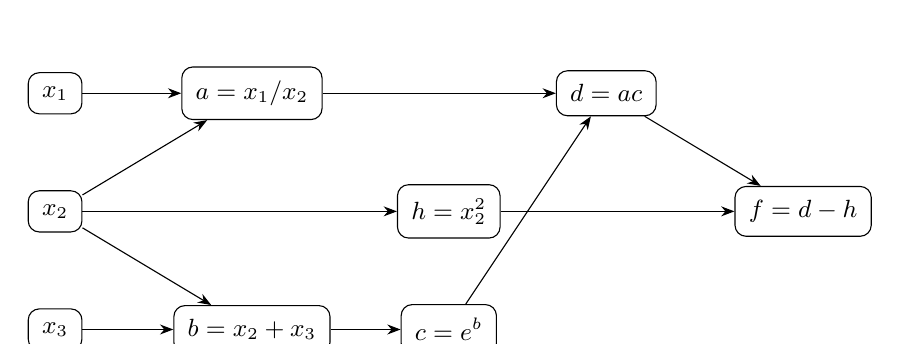
\begin{tikzpicture}[>=Stealth, every node/.style={draw, rounded corners,
  inner sep=5pt, font=\small}]
  \node (x1) at (0,1.5) {$x_1$};
  \node (x2) at (0,0) {$x_2$};
  \node (x3) at (0,-1.5) {$x_3$};
  \node (a) at (2.5,1.5) {$a=x_1/x_2$};
  \node (b) at (2.5,-1.5) {$b=x_2+x_3$};
  \node (c) at (5,-1.5) {$c=e^b$};
  \node (d) at (7,1.5) {$d=ac$};
  \node (h) at (5,0) {$h=x_2^2$};
  \node (f) at (9.5,0) {$f=d-h$};
  \draw[->] (x1) -- (a);
  \draw[->] (x2) -- (a);
  \draw[->] (x2) -- (b);
  \draw[->] (x3) -- (b);
  \draw[->] (b) -- (c);
  \draw[->] (a) -- (d);
  \draw[->] (c) -- (d);
  \draw[->] (x2) -- (h);
  \draw[->] (d) -- (f);
  \draw[->] (h) -- (f);
\end{tikzpicture}
\end{center}

\item \textbf{Computing Adjoints}
Now, compute the adjoint for each node in your computation graph with respect to $\textbf{x} = [x_1 \ \ x_2 \ \ x_3] = [1 \ \ 2 \ \ 3]$. What is the gradient with respect to $\textbf{x}$? We recommend that you use your computation graph and write it out instead of typing.
\par\smallskip
\textbf{Solution.} Let $\bar v=\partial f/\partial v$. The forward values are
\[
a=\tfrac12,\quad b=5,\quad c=e^5,\quad
d=\tfrac12e^5,\quad h=4,\quad f=\tfrac12e^5-4.
\]
Starting with $\bar f=1$, reverse propagation gives
\[
\bar d=1,\qquad \bar h=-1,\qquad
\bar a=\bar d\,c=e^5,\qquad
\bar c=\bar d\,a=\tfrac12,\qquad
\bar b=\bar c\,e^b=\tfrac12e^5.
\]
The input adjoints are obtained by summing over all outgoing paths:
\begin{align*}
\bar x_1&=\bar a\frac{1}{x_2}=\frac{e^5}{2},\\
\bar x_2&=\bar a\left(-\frac{x_1}{x_2^2}\right)
          +\bar b+\bar h(2x_2)
          =-\frac{e^5}{4}+\frac{e^5}{2}-4
          =\frac{e^5}{4}-4,\\
\bar x_3&=\bar b=\frac{e^5}{2}.
\end{align*}
Thus,
\[
\boxed{\nabla_{\mathbf{x}}f(1,2,3)=
\begin{pmatrix}e^5/2\\e^5/4-4\\e^5/2\end{pmatrix}
\approx\begin{pmatrix}74.2066\\33.1033\\74.2066\end{pmatrix}.}
\]

\end{enumerate}

\newpage
% ---------- Overview ----------
\section*{Optimizers Overview}
Adaptive gradient methods are among the most widely used optimization algorithms in deep learning. In this assignment, we focus on two main algorithms: \textbf{Adam} and \textbf{AdamW} (briefly AdaGrad, RMSProp). Because the primary sources are dense, please start with the short blog posts below, then (optionally) consult the original papers.

\paragraph*{Recommended reading (short):}
\begin{itemize}[leftmargin=1.4em]
    \item \href{https://towardsdatascience.com/understanding-deep-learning-optimizers-momentum-adagrad-rmsprop-adam-e311e377e9c2/}{Understanding Deep Learning Optimizers: Momentum, AdaGrad, RMSProp, Adam} — quick refresher on the progression from SGD to Adam.
  \item \href{https://adelbennaceur.github.io/posts/adam_vs_adamw/}{Adam vs.\ AdamW (A. Bennaceur)} — concise comparison highlighting why decoupled weight decay matters.
  \item \textbf{Supplement (Section 3):} \href{https://cs182sp21.github.io/static/discussions/dis2-sol.pdf}{CS182 Discussion 2 Solutions (Spring 2021)} — see Section~3 for a compact optimizer summary.
\end{itemize}

\paragraph*{Optional primary sources:}
\begin{itemize}[leftmargin=1.4em]
  \item \href{https://arxiv.org/abs/1412.6980}{Adam: A Method for Stochastic Optimization (Kingma \& Ba, 2015)}
  \item \href{https://arxiv.org/abs/1711.05101}{Decoupled Weight Decay Regularization (Loshchilov \& Hutter, 2017)}
\end{itemize}

Before answering the questions, also briefly review the original Adam algorithm (Algorithm 1 from Kingma \& Ba, 2014) and AdamW, reproduced below for reference.

% ---------- Adam Algorithm Block ----------
\begin{algorithm}[H]
\caption{Adam, our proposed algorithm for stochastic optimization (Kingma \& Ba, 2014)}
\begin{algorithmic}[1]
\Require $\alpha$: Stepsize
\Require $\beta_1, \beta_2 \in [0,1)$: Exponential decay rates for the moment estimates
\Require $f(\theta)$: Stochastic objective function with parameters $\theta$
\Require $\theta_0$: Initial parameter vector
\State $m_0 \gets 0$ \Comment{Initialize 1st moment vector}
\State $v_0 \gets 0$ \Comment{Initialize 2nd moment vector}
\State $t \gets 0$ \Comment{Initialize timestep}
\While{$\theta_t$ not converged}
    \State $t \gets t + 1$
    \State $g_t \gets \nabla_\theta f_t(\theta_{t-1})$ \Comment{Get gradients}
    \State $m_t \gets \beta_1 \cdot m_{t-1} + (1 - \beta_1) \cdot g_t$ \Comment{EMA of gradients}
    \State $v_t \gets \beta_2 \cdot v_{t-1} + (1 - \beta_2) \cdot g_t^2$ \Comment{EMA of squared gradients}
    \State $\hat{m}_t \gets m_t / (1 - \beta_1^t)$ \Comment{Bias-corrected 1st moment}
    \State $\hat{v}_t \gets v_t / (1 - \beta_2^t)$ \Comment{Bias-corrected 2nd moment}
    \State $\theta_t \gets \theta_{t-1} - \alpha \cdot \hat{m}_t / (\sqrt{\hat{v}_t} + \epsilon)$ \Comment{Update}
\EndWhile
\State \textbf{return} $\theta_t$
\end{algorithmic}
\end{algorithm}

\begin{algorithm}[H]
\caption{\colorbox{regpink}{Adam with L2 regularization}\; and \;
\colorbox{adamwgreen}{Adam with decoupled weight decay (AdamW)}}
\begin{algorithmic}[1]
\Require $\alpha = 0.001$, $\beta_1 = 0.9$, $\beta_2 = 0.999$, $\epsilon = 10^{-8}$, $\lambda \in \mathbb{R}$
\State \textbf{initialize} $t \gets 0$, parameter vector $\theta_{t=0} \in \mathbb{R}^n$, first moment $m_{t=0} \gets 0$, second moment $v_{t=0} \gets 0$, schedule multiplier $\eta_{t=0} \in \mathbb{R}$
\Repeat
  \State $t \gets t + 1$
  \State $\nabla f_t(\theta_{t-1}) \gets \textsc{SelectBatch}(\theta_{t-1})$
  \State $g_t \gets \nabla f_t(\theta_{t-1})\; \mathcolorbox{regpink}{+\lambda\,\theta_{t-1}}$ \Comment{(L2‐regularized Adam) add penalty inside gradient}
  \State $m_t \gets \beta_1 m_{t-1} + (1-\beta_1)\,g_t$
  \State $v_t \gets \beta_2 v_{t-1} + (1-\beta_2)\,g_t^{2}$
  \State $\hat m_t \gets m_t/(1-\beta_1^{t})$
  \State $\hat v_t \gets v_t/(1-\beta_2^{t})$
  \State $\eta_t \gets \textsc{SetScheduleMultiplier}(t)$
  \State $\theta_t \gets \theta_{t-1} - \eta_t\!\left(\alpha\,\frac{\hat m_t}{\sqrt{\hat v_t}+\epsilon}\; \mathcolorbox{adamwgreen}{+\lambda\,\theta_{t-1}}\right)$ \Comment{(AdamW) decoupled decay}
\Until{stopping criterion is met}
\State \textbf{return} optimized parameters $\theta_t$
\end{algorithmic}
\end{algorithm}

\newpage
% ---------- Questions ----------

\begin{enumerate}[label=\textbf{Q\arabic*.}, leftmargin=2.2em, resume]

  \item \textbf{Reviewing Previous Optimizers.}  
   We have learned how variants of gradient descent improve training speed and stability.  
  For each method --- \textbf{Momentum}, \textbf{AdaGrad}, and \textbf{RMSProp} --- write the update equations, state the key idea (one concise sentence), and describe the problem it solves (one concise sentence).  
  We have provided SGD for you.

  \textbf{SGD} \\
\emph{Update:} $\theta_t \gets \theta_{t-1} - \alpha\, g_t$, where $g_t = \nabla_\theta f_t(\theta_{t-1})$. \\
\emph{Key idea:} Use a random minibatch each step for computational efficiency. \\
\emph{Problem it solves:} Full-batch gradient descent is slow and redundant; minibatching makes updates cheaper.
\par\smallskip
\textbf{Solution.} All operations below are elementwise, $g_t=\nabla f_t(\theta_{t-1})$,
and all accumulators start at zero.

\textbf{Momentum:}
\[
u_t=\beta u_{t-1}+g_t,\qquad \theta_t=\theta_{t-1}-\alpha u_t.
\]
\emph{Key idea:} Accumulate an exponentially decaying history of gradients.
\emph{Problem it solves:} It reduces oscillation and accelerates progress along directions with consistent gradients.

\textbf{AdaGrad:}
\[
s_t=s_{t-1}+g_t^2,\qquad
\theta_t=\theta_{t-1}-\alpha\frac{g_t}{\sqrt{s_t}+\epsilon}.
\]
\emph{Key idea:} Scale each coordinate's update by its accumulated squared gradients.
\emph{Problem it solves:} It adapts to unequal gradient scales and gives infrequently updated coordinates relatively larger effective learning rates.

\textbf{RMSProp:}
\[
s_t=\beta s_{t-1}+(1-\beta)g_t^2,\qquad
\theta_t=\theta_{t-1}-\alpha\frac{g_t}{\sqrt{s_t}+\epsilon}.
\]
\emph{Key idea:} Use an exponential moving average of squared gradients to adapt each coordinate's step size.
\emph{Problem it solves:} It avoids AdaGrad's continually growing accumulator and the resulting continual decay of effective learning rates.


  \item \textbf{Handling Large Gradients.} What happens when gradients are very large in plain gradient descent, and how does Adam’s update rule address this issue?
  \par\smallskip
\textbf{Solution.} Large gradients in plain gradient descent can cause oversized updates,
overshooting, oscillation, or divergence.
Adam smooths gradients with momentum and divides the update by
$\sqrt{\hat v_t}+\epsilon$, reducing the effective learning rate in coordinates
with large recent squared gradients; this mitigates oversized steps but does not guarantee stability.


  \item \textbf{Introducing AdamW.} How does AdamW decouple weight decay from the gradient update? Why does this help generalization?
  \par\smallskip
\textbf{Solution.} AdamW computes Adam's moments using only the loss gradient and applies
weight decay separately:
\[
\theta_t=(1-\alpha\lambda)\theta_{t-1}
-\alpha\frac{\hat m_t}{\sqrt{\hat v_t}+\epsilon}.
\]
The decay is not accumulated in the moments or rescaled by the adaptive denominator,
so it provides more predictable regularization that can discourage large weights and reduce overfitting.
Here $\lambda$ follows the learning-rate-scaled convention in Q8.


  \item \textbf{AdamW Weight Decoupling.} How does decoupling weight decay affect hyperparameter sensitivity?
  \par\smallskip
\textbf{Solution.} Decoupling prevents the strength of weight decay from depending on
Adam's gradient history and coordinatewise scaling, making the decay coefficient
easier to tune separately from the adaptive update.
This reduces hyperparameter interactions, but does not eliminate them: under
the convention in Q8, the per-step shrinkage still depends on $\alpha\lambda$.


  \item \textbf{Tracing Adam’s Origins (Line Mapping).}   
    As seen in lecture, Adam builds on ideas from several earlier optimizers. Now let's explore exactly how these ideas are used in Adam. Below are the key lines (7–11) from the Adam algorithm.  
    
    For each line, label which previous algorithm inspired it (or indicate if it was newly introduced) using one of the following categories:
    \begin{itemize}
        \item Momentum
        \item Adaptive Scaling (RMSProp/AdaGrad)
        \item Newly Introduced by Adam
        \item Combination (merges two or more earlier ideas into a single update rule)
    \end{itemize}

    Briefly explain your reasoning for each label.

    \begin{algorithm}[H]
    \caption{Adam: Core Update Lines (Kingma \& Ba, 2014)}
    \begin{algorithmic}[1]
        \State $m_t \gets \beta_1 m_{t-1} + (1 - \beta_1) g_t$ \Comment{Line 7}
        \State $v_t \gets \beta_2 v_{t-1} + (1 - \beta_2) g_t^2$ \Comment{Line 8}
        \State $\hat{m}_t \gets m_t / (1 - \beta_1^t)$ \Comment{Line 9}
        \State $\hat{v}_t \gets v_t / (1 - \beta_2^t)$ \Comment{Line 10}
        \State $\theta_t \gets \theta_{t-1} - \alpha \cdot \hat{m}_t / (\sqrt{\hat{v}_t} + \epsilon)$ \Comment{Line 11}
    \end{algorithmic}
    \end{algorithm}
    \par\smallskip
\textbf{Solution.}
\begin{itemize}[leftmargin=1.4em]
\item Line 7: \textbf{Momentum}; it accumulates an exponential moving average of gradients.
\item Line 8: \textbf{Adaptive Scaling (RMSProp/AdaGrad)}; the moving average of squared gradients supplies coordinatewise scale estimates.
\item Line 9: \textbf{Newly Introduced by Adam} (among the compared methods); it corrects the first moment's initial bias toward zero.
\item Line 10: \textbf{Newly Introduced by Adam} (among the compared methods); it corrects the second moment's initial bias toward zero.
\item Line 11: \textbf{Combination}; it combines the momentum numerator with adaptive scaling by the root second moment.
\end{itemize}


\newpage
\item \textbf{Step 1 Gradient: Adam and AdamW updates.}
Consider the scalar objective
\[
f(\theta) = \theta^2, \qquad \nabla_\theta f(\theta) = g_t = 2\theta_t.
\]
Use the following hyperparameters unless otherwise specified:
\[
\theta_0 = 10,\quad \alpha = 0.1,\quad \lambda = 0.01,\quad 
\beta_1 = 0.9,\quad \beta_2 = 0.99,\quad \epsilon = 10^{-8},\quad 
m_0 = v_0 = 0.
\]
Compute all quantities for $t=1$.
\begin{enumerate}[label=(\alph*)]
  \item Compute $g_1, m_1, v_1$.
  \item Compute bias-corrected $\hat m_1, \hat v_1$ (feel free to refer to Algorithm Block provided in Q1).
  \item Compute $\theta_1^{\text{Adam}} = 
        \theta_0 - \alpha \frac{\hat m_1}{\sqrt{\hat v_1} + \epsilon}$ (step 1 update of Adam).
  \item Compute $\theta_1^{\text{AdamW}} =
        \theta_1^{\text{Adam}} - \alpha \lambda \theta_0$ (step 1 update of AdamW).
\end{enumerate}

\par\smallskip
\textbf{Solution.} Evaluate the first gradient at $\theta_0$ (in general,
$g_t=2\theta_{t-1}$ for an update indexed by $t$).
\begin{align*}
\text{(a)}\quad &g_1=20,\quad m_1=0.1(20)=2,\quad v_1=0.01(20^2)=4.\\
\text{(b)}\quad &\hat m_1=2/(1-0.9)=20,\quad \hat v_1=4/(1-0.99)=400.\\
\text{(c)}\quad &\theta_1^{\mathrm{Adam}}=10-0.1\frac{20}{20+10^{-8}}\approx9.9.\\
\text{(d)}\quad &\theta_1^{\mathrm{AdamW}}=\theta_1^{\mathrm{Adam}}-0.1(0.01)(10)\approx9.89.
\end{align*}

\item \textbf{Step 2 Gradient: Adam continuation ($\beta_2 = 0.99$).}
Compute the second update step for Adam (you don't have to compute for AdamW). In other words, compute $\theta_2^{\text{Adam}}$.
\par\smallskip
\textbf{Solution.} Continuing from Adam's $\theta_1\approx9.9$ (not AdamW's value),
\begin{align*}
g_2&=2\theta_1\approx19.8,\\
m_2&=0.9(2)+0.1(19.8)=3.78,\\
v_2&=0.99(4)+0.01(19.8^2)=7.8804,\\
\hat m_2&=\frac{3.78}{1-0.9^2}\approx19.894737,\qquad
\hat v_2=\frac{7.8804}{1-0.99^2}=396,\\
\theta_2^{\mathrm{Adam}}&=9.9-0.1\frac{19.894737}{\sqrt{396}+10^{-8}}
\approx\boxed{9.800025}.
\end{align*}


\item \textbf{Conceptual reflection.}
Keep the baseline at $\beta_2 = 0.99$. Now imagine we set $\beta_2 = 0.5$ (all else unchanged).
Without redoing the full calculation, explain qualitatively what changes at $t=1$ and $t\ge2$,
and how this would affect stability vs.\ responsiveness.

\par\smallskip
\textbf{Solution.} At $t=1$, $v_1$ increases when $\beta_2$ decreases, but
$\hat v_1=(1-\beta_2)g_1^2/(1-\beta_2)=g_1^2$, so the corrected moment and parameter update are unchanged.
For $t\ge2$, $\beta_2=0.5$ gives recent squared gradients more weight; in this example the gradients decrease, so the second-step denominator is slightly smaller and the update is slightly larger.
The estimate responds faster to changes but smooths noise less, so step sizes can fluctuate more than with $\beta_2=0.99$.

\end{enumerate}

\end{document}
